\documentclass[10pt,twocolumn,letterpaper]{article}

\usepackage{cvpr}
\usepackage{times}
\usepackage{epsfig}
\usepackage{graphicx}
\usepackage{amsmath}
\usepackage{amssymb}

% Include other packages here, before hyperref.

% If you comment hyperref and then uncomment it, you should delete
% egpaper.aux before re-running latex.  (Or just hit 'q' on the first latex
% run, let it finish, and you should be clear).
\usepackage[breaklinks=true,bookmarks=false]{hyperref}

\cvprfinalcopy % *** Uncomment this line for the final submission

% Pages are numbered in submission mode, and unnumbered in camera-ready
%\ifcvprfinal\pagestyle{empty}\fi
\setcounter{page}{1}
\begin{document}

%%%%%%%%% TITLE
\title{Object Detection and Tracking Pipeline}

\author{Pranav Jain\\
Person Number: 50208349\\
UBIT: pjain4\\
%{\tt\small firstauthor@i1.org}%
% For a paper whose authors are all at the same institution,
% omit the following lines up until the closing ``}''.
% Additional authors and addresses can be added with ``\and'',
% just like the second author.
% To save space, use either the email address or home page, not both
\and
Muthuvel Palanisamy	\\
Person Number: 50246815\\
UBIT: muthuvel\\
%{\tt\small secondauthor@i2.org}%
\and
Manvijay Lather	\\
Person Number: 50200437\\
UBIT: manvijay\\
%{\tt\small secondauthor@i2.org}%
}

\maketitle
%\thispagestyle{empty}

%%%%%%%%% ABSTRACT
\begin{abstract}
   Object detection and tracking have become an integral part of Computer Vision. Efficient realization of these techniques in images and videos have helped create various applications in the field of automation, face detection, motion capture etc. This paper implements\footnote{Code can be found at \url{https://github.com/pranav9056/Object-tracking}} an object tracking pipeline using Lucas-Kanade tracker after being initialized by tensorflow's object detection API and compares this technique to tracking using just the object detection API at each frame. We also look at a hybrid approach where object detection is used multiple times. 
   \end{abstract} 
%%%%%%%%% BODY TEXT
\section{Literature Review}

An optimal approach to any tracking algorithm is based on two key areas in computer vision; object detection and object tracking. While a variety of methods are available for accomplishing these techniques, not all of them prove to be effective in achieving a significant efficiency. Conventional method for object detection and tracking makes use of techniques such as Frame Differencing, Optical flow, Background subtraction, Point-tracking techniques, SVM and Kernel based tracking. A brief introduction to a some of these techniques is given below

%-------------------------------------------------------------------------

\subsection{Frame Differencing}
Frame differencing suggests calculating the difference between two successive frame in an image to find the moving objects. While the idea is simple and east to implement, it is generally considered ineffective in dynamic environments where the changes in the frame of an image are not just isolated to the objects that needs to be tracked.

\subsection{Background Subtraction}
This techniques involves modelling the background and use that for background subtraction. We must choose a background model sensitive enough to uncover the objects in an image/frame and use that as a reference in tracking. This can be done by find the variation between frames and the reference models. Common filters like mean and median filters can be used to calculate the difference in pixel intensities. This is mainly achieved using recursive and non-recursive algorithms. A background subtraction algorithm based on frame differencing is explored in ~\cite{literaturereview}.  Similar to the previous approach, this method becomes in effective in the variation in the background becomes high. A more sophisticated method which can ignore highly changing  background will be needed for detecting objects will be required for advanced models.

\subsection{Support Vector Machine (SVM)}
SVMs apply machine learning algorithms for learning, analyzing and storing the the output as positive and negative values that represent the tracked objects in an image and objects not tracked in an image. SVMs have a wider range of application in real world, that includes but not isolated to face detection, bioinformatics, handwriting or pattern recognitions etc.

\subsection{Silhouette Based Tracking approach}
This approach is helpful in tracking complex geometric shapes present in images such as hands, fingers etc. It can be done by employed by track either the boundary(Contour) of objects in an image or the shape corresponding to those objects. Contour based tracking can be achieved using gradient descent minimization technique and using state space models to trace boundaries. Shape Matching is a kind of brute force approach applied on a region of interest in a frame to identify objects that can be matched with a reference object


\subsection{Tensorflow API}

Tensorflow was originally developed by Google Brain Team to help facilitate machine learning and deep learning researches. Tensorflow's object detection model consists of a neural network trained from COCO(Common Objects in Context) dataset. It contains around 300k images of 90 commonly used objects. The library consists of 5 different models that can be used; classified based on their speed and accuracy of placing the bounding box (a box that encloses a detected object). We plan to use the latest version of one of the models - \textit{ssd\textunderscore mobilenet\textunderscore v1\textunderscore coco}, which has the highest speed while sacrificing a little efficiency in placing the bounding box on the object.

\subsection{Lucas-Kanade Tracker in OpenCV}

Developed by Bruce D. Lucas and Takeo Kanade, Lucas-Kanade Tracker uses an optical flow algorithm to track an object in subsequent frames. OpenCV incorporates a predefined function - \textit{calcOpticalFlowPyrLK()} , that implements this algorithm. We will use this function in our object tracking pipeline.





%-------------------------------------------------------------------------
\section{Method Proposed}
Neural Networks have been proven to produce better and efficient detection models. 

Our idea was to come up with an ideal tracking pipeline that is able to self detect objects and track them. Given the scope of the problem we decided to make use of TensorFlow's object detection library which provided us with a desired pre-trained model and OpenCV's implementation of Lucas Kanade Tracker.  

We experiment with three different techniques for achieving a tracking algorithm which are described in this section.

\subsection{Objection detection using Tensorflow}
In this method, we use TensorFlow's object detection model to perform tracking completely. The method starts by detecting objects present in the first frame of a video or image by using a model pre-trained on the COCO Dataset. The object detected is visualized using a bounding box enclosing the object. This is done by the function  \textit{visualize\textunderscore boxes\textunderscore and\textunderscore labels\textunderscore on\textunderscore image\textunderscore array()}  In every successive frame, the same object detection algorithm is employed to detect the interesting objects in the frame. To summarize, detecting  objects in all the frames individually translates to an indirect object tracking method.

\subsection{Object tracking initialized by Tensorflow}

In this method, we initialize the process by starting with Tensorflow's object detection. This part of the algorithm detects the objects of interest in the image using a pre-trained model same as the one in the previous method. This is done till the objects detected in the frames are above a certain confidence level. The objects are later used as input for tracking in the second part.

The object detection technique employed here returns an array of bounding boxes which consists of an array of co-ordinates for boxes enclosing the objects and their corresponding scores. Since, all the boxes detected may not be ideal, we set a threshold to the scores to limit the number of objects. This is done by calling \textit{findBoxes()} which was added by us and returns a boolean variable that marks object detection. 

In the next part, we use SIFT detectors on the first frame of the video/ image where an object was detected to find the feature points in that image. Not all points here are required for tracking. Hence, we limit them by choosing only the feature points present inside the bounding box detected from the object detection. This gives us the keypoints that can be used to track the object in subsequent frames.

Using the feature points extracted above, we track these points by using - \textit{calcOpticalFlowPyrLK()} from openCV, which provides an implementation of Lucas-Kanade Tracker. The difference in the location of the object in the current frame to that in the previous frame in calculated. This is used to eliminate static objects from background by discarding all points that are below a threshold. 

Finally, a bounding box is drawn over the object using the \textit{visualize\textunderscore boxes\textunderscore and\textunderscore labels\textunderscore on\textunderscore image\textunderscore array()}  function from tensorflow library.



\subsection{Hybrid Approach}
As the name suggests, this method is a mixture of both the methods mentioned above. The idea is to combine Tensorflow's efficiency in detection and the speed of tracking achieved by KLT algorithm. Using this approach we can strengthen the current belief of the objects. 

Instead of just using the object detection technique only for initialization, we use Tensorflow to detect object after every \textbf{N} frames and pass the detected objects as input to tracker as in the second approach.  To summarize once the object detection passes the input to tracker, it tracks the objects for the next \textit{N} frames after which it detects objects again and passes them to the tracker. This approach has a potential benefit of detecting objects that are not present in the beginning of the video. Also, it could help rectify any pitfalls in the Tracking algorithm by periodically running object detection again while still maintaining the speed.

%------------------------------------------------------------------------
\section{Experimental Analysis and Result}

We have tested all the three approaches discussed earlier with a few  videos and image sets from real datsets. A link to the the original output files are in ~\cite{Videolink}. Also, we have compared the time taken to track an object in a video using three different approaches discussed in the previous sections of this report. This section gives a detailed analysis of the three methods and mentions their advantages and pitfalls.

\subsection{Object detection using tensorflow}  

When we implemented the first algorithm (Object Detection using Tensorflow) on the videos, we found out that it misses on detecting objects later in the video which were detected in the initial frames of the video  (\textit{See Figure 1}). We tried it on a set of test images of a traffic signal and observed something similar with the car 
 (\textit{Figure 2}). This loss of detection can perhaps be due to occlusion/loss in some features. As far as the running time is concerned this approach almost took twice as long as the other two algorithms since objects were being detected at each frame.

    %% Inluding the images
\begin{figure}
\includegraphics[width=\linewidth]{Detection.jpg}
\caption{Detection using Tensorflow for a video }
\end{figure}


\begin{figure}
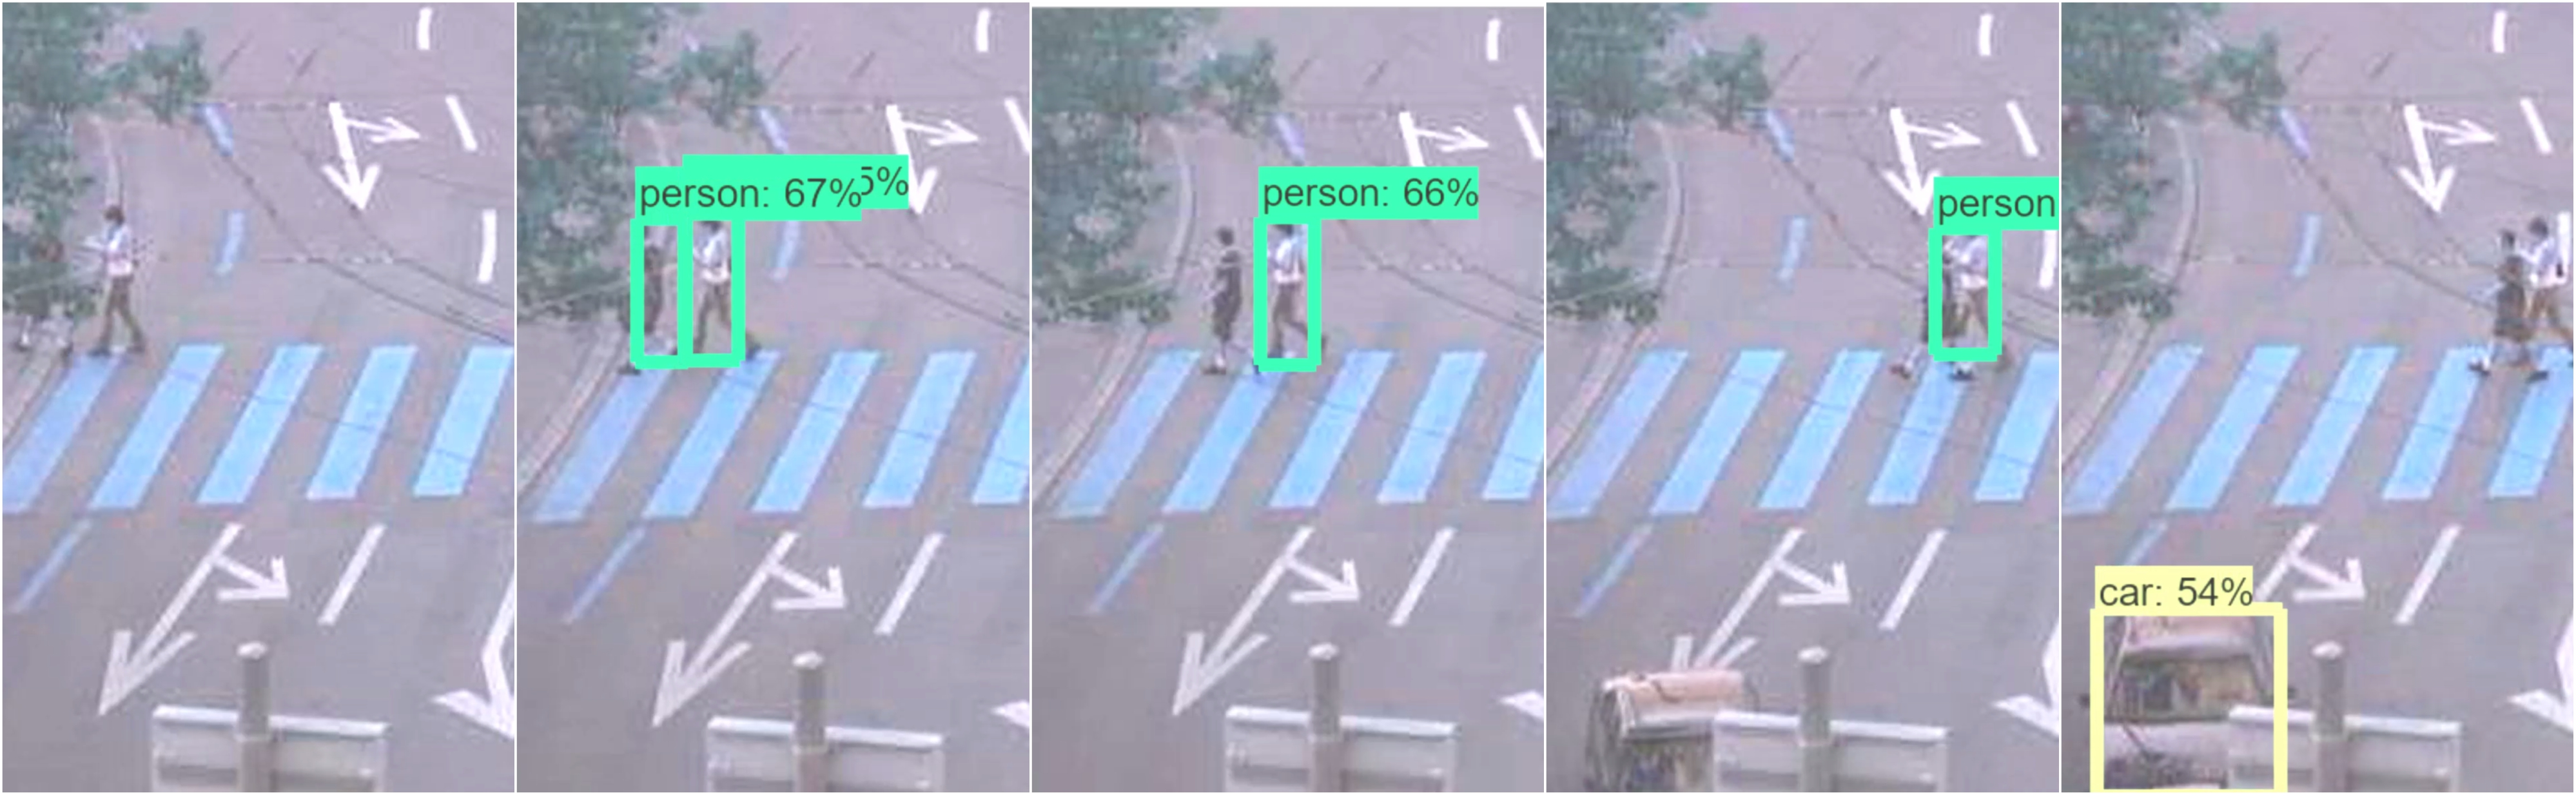
\includegraphics[width=\linewidth]{Detection_images.jpg}
\caption{Detection using Tensorflow for a sequence of images}
\end{figure}

\textbf{Advantages:}

This is the backbone of the other two approaches.
Tensorflow provides an easy to use object detector which can be used right off the shelf without having to train the models. This will also detect the most number of objects even if it can't always keep track of them.

\textbf{Disadvantages:}

When run on videos, doesn’t always detect the object which was detected in one of the previous frames of the same video. 
It takes more time.

\subsection{Object tracking initiated by Tensorflow}  

On implementing this algorithm, we got quicker results than the first approach, almost half the time. The other positive point of this algorithm we observed was that it never lost track of the object which was tracked in the initial frames of the video. However, there is a limitation in this algorithm. The box enclosing the feature points of the detected objects keep reducing in the size as the video progresses. The reason for that diminishing box is the lesser number of feature points left inside the box after comparing two consecutive frames.\textit{ See Figure 3}.
Also the objects that are tracked depend completely on the frame in which they were detected, that is it misses out on the objects that could have been later detected by the object detector.

\begin{figure}
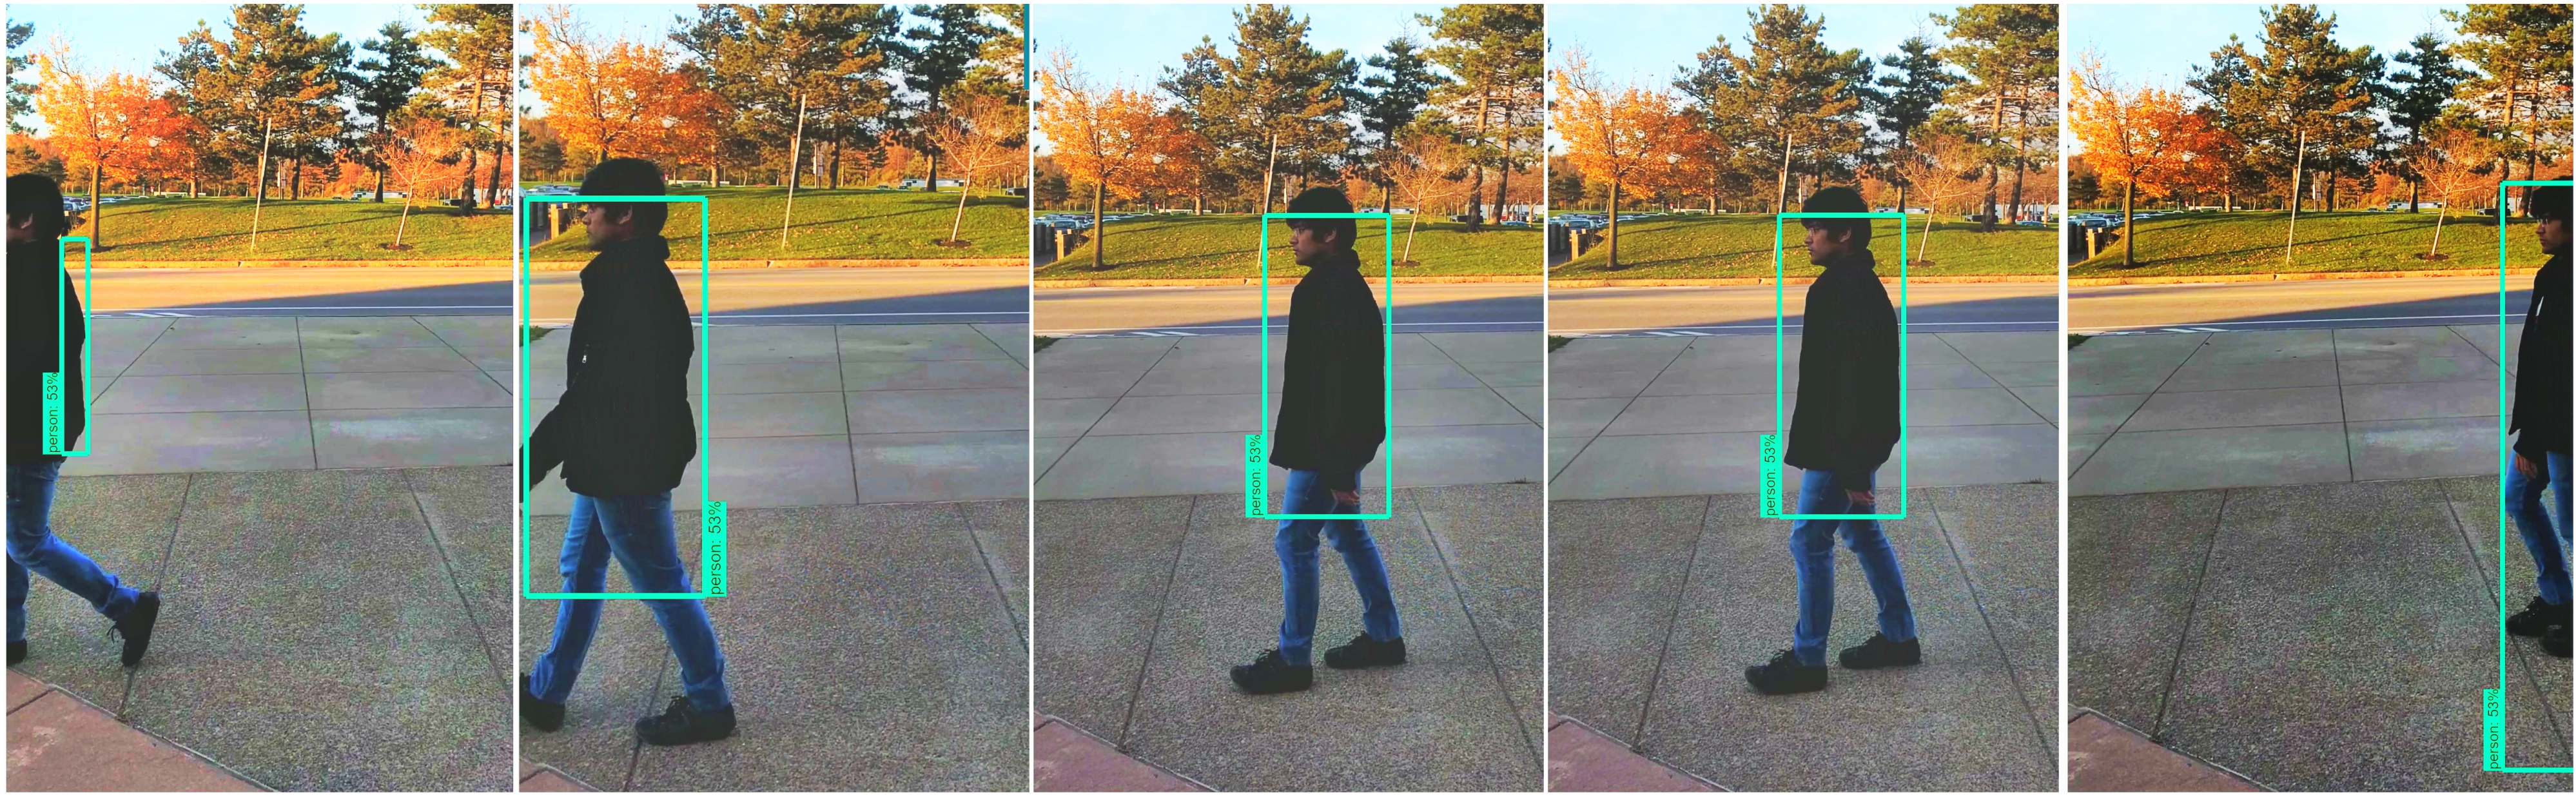
\includegraphics[width=\linewidth]{Tracking.jpg}
\caption{Object Tracking in a video initiated by Tensorflow}
\end{figure}

This algorithm was run on a series of test images as well, screenshots of which are shown in \textit{Figure 4}.

\begin{figure}
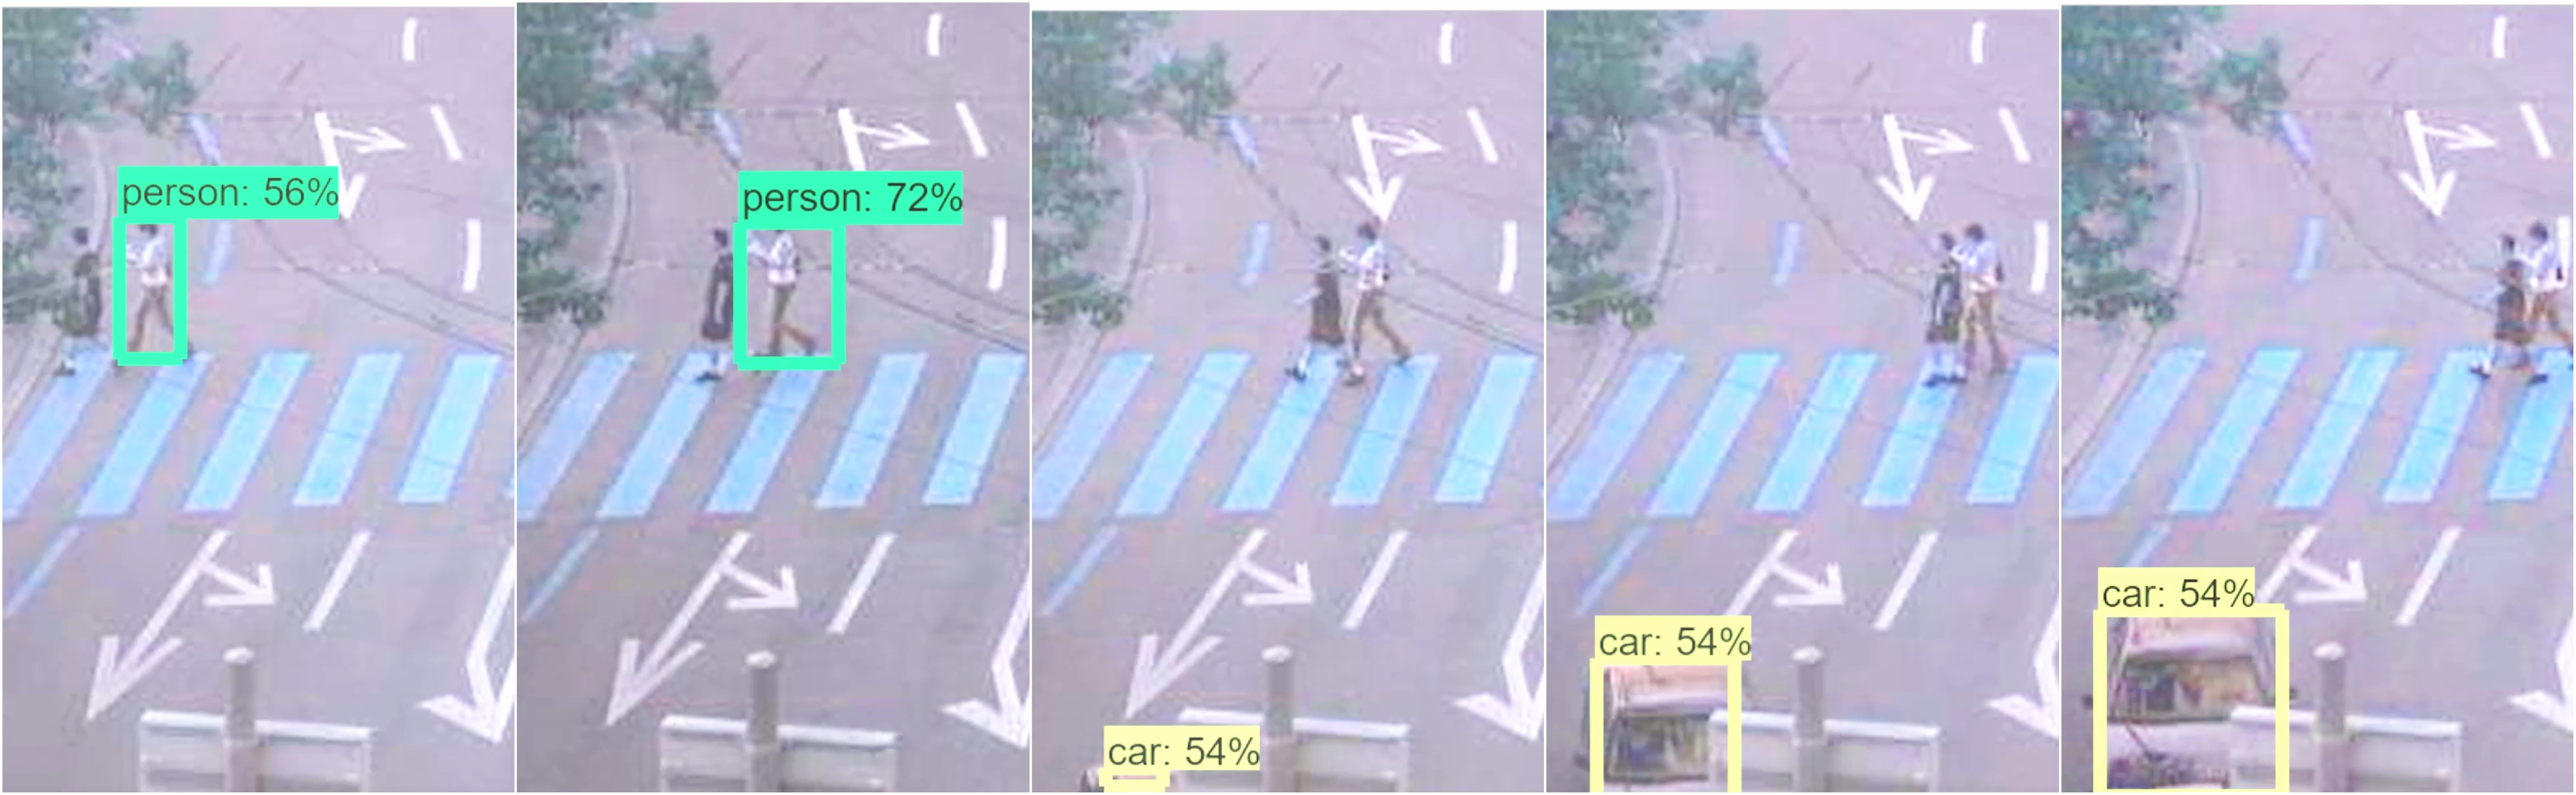
\includegraphics[width=\linewidth]{Tracking_images.jpg}
\caption{Object Tracking in a sequence of images initiated by Tensorflow}
\end{figure}

\textbf{Advantages:}

•	It is substantially faster than TensorFlow approach and marginally faster than Hybrid approach.
•	It keeps track of the object detected in one frame till the end of the video.

\textbf{Disadvantages}

•	Tracks only the objects detected in one frame throughout the video.
•	Decrease in size of the box enclosing the feature points of the detected object as the time passes or in other not enclosing all the feature points of the detected object after a few frames.
 
\subsection{Hybrid Approach}  

This approach keeps the best elements from the previous algorithms. It is almost as fast as second approach and can be trusted with detecting new objects in the middle of the video (a trait shown by first algorithm). However, the only limitation it has is its over reliance on Tensorflow which leads to not being able to track objects once Tensorflow is unable to detect the object. It’s an upgrade on tracking algorithm as it detects new objects even in the intermediate frames of the video but loses its edge if TensorFlow fails to detect objects in the frame where this algorithm uses TensorFlow for detection. \textit{See Figure 5}.

    %% Inluding the images
\begin{figure}
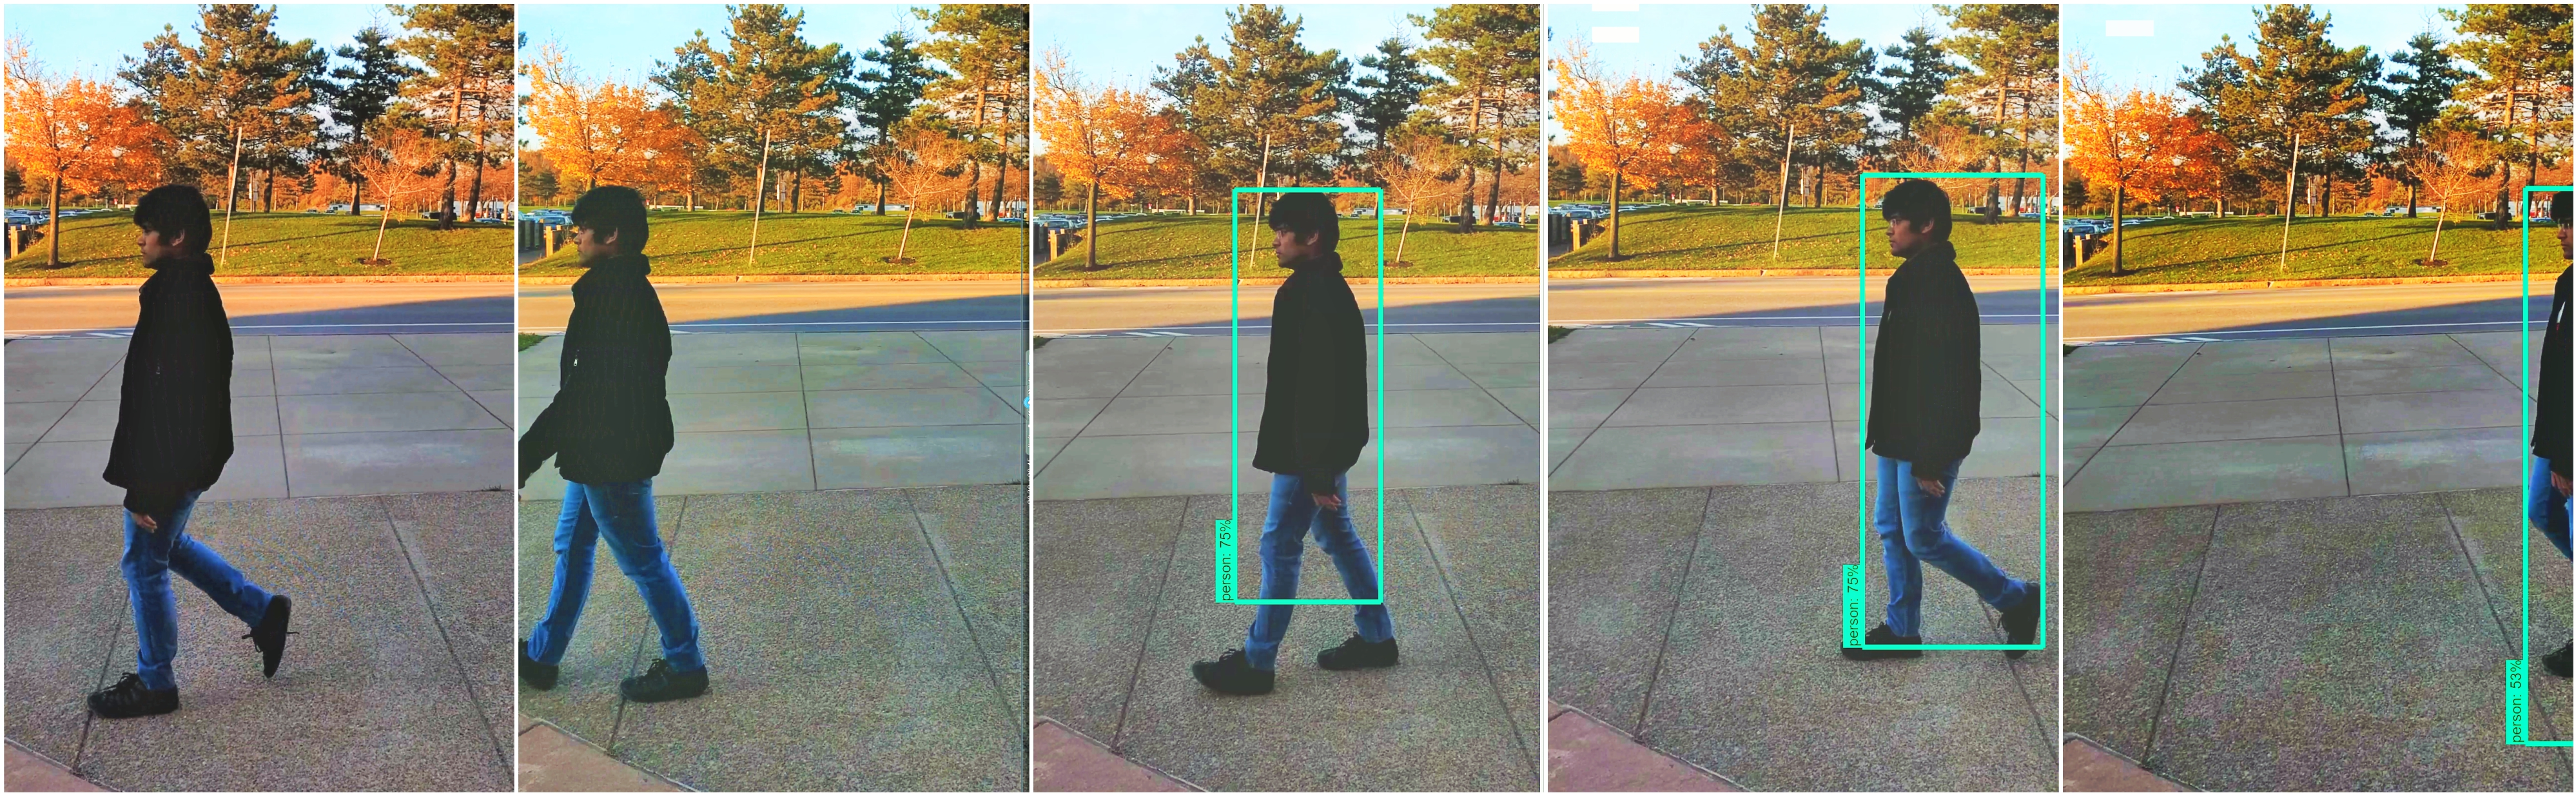
\includegraphics[width=\linewidth]{Hybrid.jpg}
\caption{Hybrid approach on a video}
\end{figure}

This algorithm was run on a series of test images as well, screenshots of which are shown in \textit{Figure 6}.

    %% Inluding the images
\begin{figure}
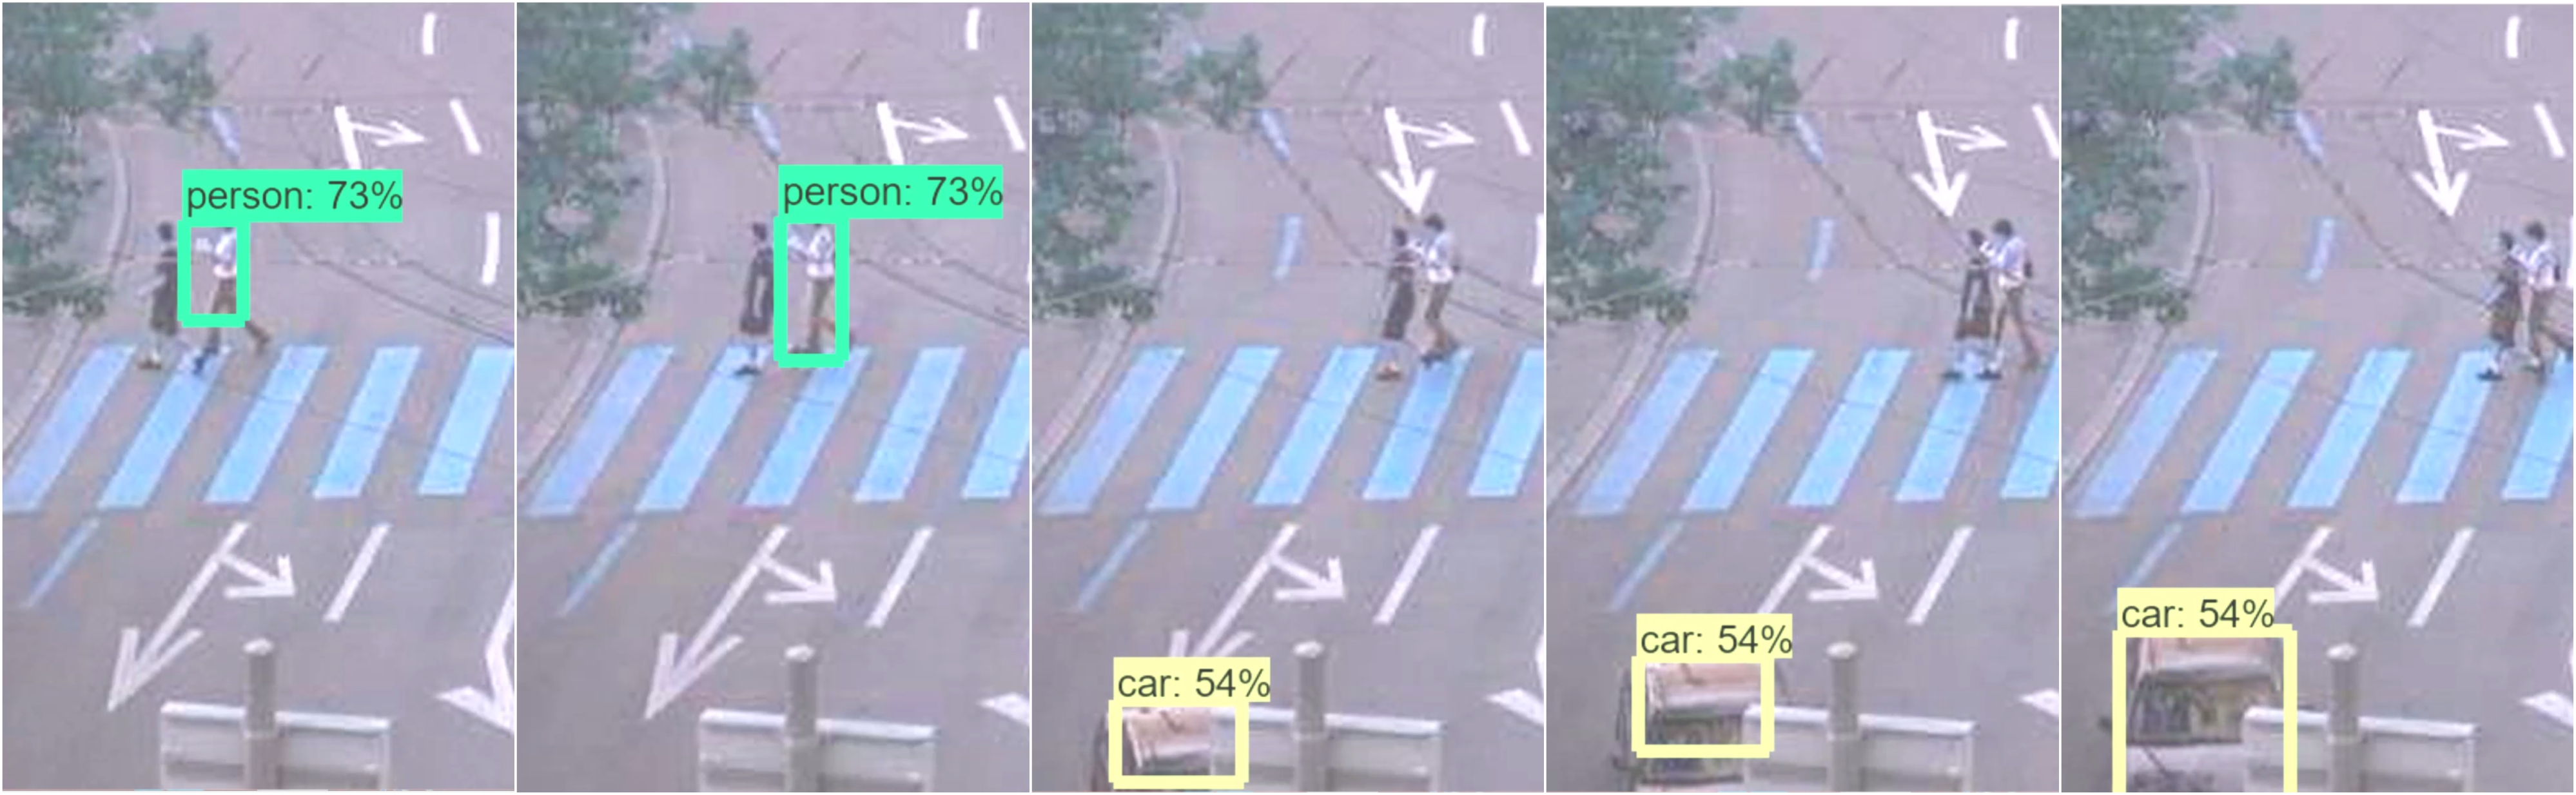
\includegraphics[width=\linewidth]{Hybrid_images.jpg}
\caption{Hybrid approach on a sequence of images}
\end{figure}

\textbf{Advantages:}

•	Faster than TensorFlow/Object Detection approach.
•	Has more chance of tracking new objects.

\textbf{Disadvantages:}

•	May loose track of objects that it was tracking due to re initialization of object detection. The frame at which it is reinitialized plays an important factor and can be different for different videos.

\subsection{Comparison of different methods}


The graph shown in \textit{Figure 7} represents the data we gathered after running these three algorithms on 3 different videos of same length, i.e. 3 seconds each. It can be clearly seen that the the first approach is time consuming and the other two have comparable running times.  


    %% Inluding the images
\begin{figure}
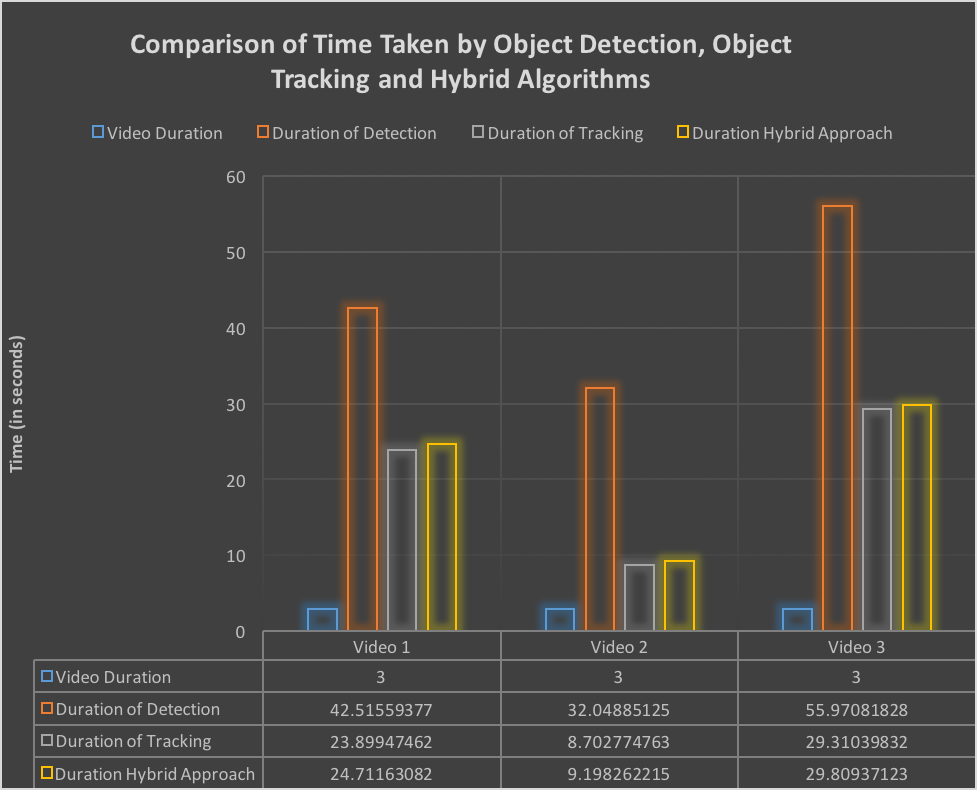
\includegraphics[width=\linewidth]{Graph.png}
\caption{Graph of Time Vs Technique}
\end{figure}
  
 
%-------------------------------------------------------------------------

\section{Conclusion and Future Work}

In Conclusion, We feel that this was really good starting point
to acquaint ourselves to the existing tracking algorithms. This project was feasible as it relied on open source code while at the same time exposed us to new API's

As mentioned earlier, Tensorflow has 5 pre-trained models for object detection of which we had used only the one. We wish to experiment with the remaining four models and see how these models fare with respect to the existing design. 

To overcome the shortcomings of the pipeline, we will be looking at other alternatives for object detection. The primary reason for this is to reduce the chance of error and increase accuracy while detecting objects. Tensorflow though faster and effective most of the time, fails to detect objects at certain frames which when coinciding with the object detection frame, can prove to hamper the tracking process.

As mentioned before, hybrid approach, did not meet our expectations fully. This is because the sweet spot for re-initializing object detection varies for different videos. Perhaps we can use a couple of consecutive frames to detect objects instead of going with the first frame where objects are detected, this or a different objection detection technique as suggested above might make the hybrid approach more robust and is left for future work.

Also, we plan on running SIFT detector only inside the bounding box of the detected region of the object and hope that it produces a positive impact on the speed on our implementation.





%-------------------------------------------------------------------------
\begin{thebibliography}{9}
\bibitem{research1} 
\url{https://research.googleblog.com/2017/06/
supercharge-your-computer-vision-models.html}
 
\bibitem{HW} 
\url{http://16720.courses.cs.cmu.edu/hw/hw3.pdf}
 
\bibitem{research} 
\url{https://towardsdatascience.com/building-a-real-time-object
-recognition-app-with-tensorflow-and-opencv-b7a2b4ebdc32}

\bibitem{literaturereview}
Rupali S.Rakibe, Bharati D.Patil.
\textit{Background Subtraction Algorithm Based Human Motion Detection}. 
International Journal of Scientific and Research Publications, May 2013

\bibitem{Videolink} 
\url{https://goo.gl/F5MFyF}

\end{thebibliography}


%-------------------------------------------------------------------------



%-------------------------------------------------------------------------
\


{\small
\bibliographystyle{ieee}
\bibliography{egbib}
}

\end{document}
